\documentclass[times, 11pt, twocolumn]{article}
\usepackage[latin1]{inputenc}
\usepackage{amsmath,amstext,amsfonts,amssymb}
\usepackage{times}
\usepackage{epsfig,float}
\usepackage{graphicx}
\usepackage{caption}
\usepackage{subcaption}
\usepackage{url}
\usepackage{rotate}
\usepackage{rotating}
\usepackage{array}
\usepackage{algorithm}
\usepackage{algorithmic}
\usepackage[usenames,dvipsnames]{color}
\usepackage{colortbl}
\usepackage[margin=0.7in]{geometry}

\DeclareMathOperator*{\bow}{bow}
\DeclareMathOperator*{\simil}{sim}


%\pagestyle{empty}

\begin{document}

\title{Detecting and Characterizing Deceptive Tweets}
\author{Alex Kantchelian and Sebastian Benthall \\
University of California, Berkeley \\
 \texttt{\{akant@cs,sb@ischool\}.berkeley.edu}\\
 }
 \date{}

\maketitle

\begin{abstract}
	In this work, we consider the problem of ``deceptive tweets'', e.g. tweets 
	linking to at least one URL and such that the tweet content is not related 
	to the URL content. We describe an LDA-based method for detecting deceptive 
	tweets and evaluate its performance on a random sample of about 210k tweets from 
	October 2010. We use this evaluation to gain some insight into the deceptive 
	tweets issue. As an interesting by product, our work resulted in an efficient, 
	information theoretic language detection algorithm for short character runs.
\end{abstract}

\section{Introduction}

Links can hold surprises. In social media especially, users encounter links in fleeting 
messages that may contain little context, if any. This environment enables deception in 
the presentation of links, as the linked content may only share little in common, if any, 
with the original message. Socially, deception can be a game, as in the rick-rolling prank [???], 
whereby a user claims to be sharing a serious article but instead links to a dated music 
video. Aside from such recreational instances, how prevalent are deceptive messages and 
what are their relation to spam? Our study investigates this connection in the context of Twitter.

We operationalize deception as the similarity between a tweet containing a link 
and the content of the HTMLs to which the link resolves. As deception involves an element 
of subjective interpretation, we first use an algorithmic method of approximating latent 
semantic structure: topic modeling. Topic models provide a means for dimensionality reduction 
of lexical features in a way that can capture interpretable categories of content \cite{Blei2003}.

Our guiding hypothesis is that spammy tweets will have more dissonance between their 
contextual information and linked content. We test this hypothesis using data provided by the 
Monarch project \cite{Thomas2011}. This data bundles information about tweets containing 
links with the crawled HTML of the pages linked to. These bundles are labeled as spam or 
ham based on the links' presence on URL blacklists.

We show that indeed, there is a significant, albeit quite noisy, relationship between content
dissonance and the spaminess character of tweets. We manually identify the causes of noise 
and explain how to address them in an ulterior iteration of the project. This suggests that
a content dissimilarity measure might be a useful feature for spam detection. In this perspective,
we finally briefly discuss the robustness of the feature in the face of adversity.

In the process of developing our method, we created a high-performance language detection 
algorithm for short texts that we describe alongside the other processing steps.

\section{Related Work}
\subsection{Spam Detection}
In general, previous work on spam detection for social networks has strongly favored 
either content or envelope based features. In the content-based approaches, \cite{Cormack2007} 
demonstrates that spam filtering based on lexical, message content level features 
for short messages is surprisingly effective through a comparison of several machine 
learning algorithms across multiple corpora. On the other side of the spectrum, \cite{Stringhini2010} 
tackles the problem of spam accounts detection on general social networks by using graph 
related features (number of friends, contact requests, \dots), regardless of actual 
message content. \cite{Zhang2011}, \cite{Ghosh2011} have shown that envelope features 
such as timing data are informative in classifying automated or semi-automated behavior 
on Twitter. \cite{Gao2010} has brushed the picture of spam campaigns on Facebook, by grouping 
wall posts by shared URLs and contents, and then detecting spam clusters by simple 
burstiness and distributeness heuristics.

As both a middle ground and a demonstration of technical feasibility, \cite{Thomas2011} 
developed a real-time service for detecting whether a URL linked to from email or 
social media is spam. Their system, Monarch, collects features from the linked page 
using an instrumented browser and then performs classification using a novel architecture 
designed for scale. In their analysis, they provide metrics for the salience of 
features for spam detection.

\subsection{Topic modeling}
Prior spam filtering research on Twitter employs myriad classification algorithms. We hope 
to make a contribution by using topic modeling methods, originally from natural language 
processing, designed to statistically infer latent semantic structure or generative features 
from a corpus. \cite{Blei2003} first introduced Latent Dirichlet Allocation, a probabilistic 
graphical model whose hidden, also called latent, variables, the topics, are distributions 
over the explicit features, the words or tokens. Once these hidden variables have been 
inferred from a corpus, that topic model can then be used to derive a topic mixture vector 
for new documents, reducing it to a lower-dimensional feature space.

LDA has previously been successfully applied to social network data. \cite{Hong2010} 
compares different methods of aggregating tweets to compensate for the short message 
length. Their results suggest that when evaluating the behavior of users, it is better to 
train topic models on documents composed of the users' aggregated messages as opposed to 
individual messages. \cite{Ramage2010} compensates for short message length by using a 
partially supervised variant, Labelled LDA, where some tokens were pre-identified as 
topic labels. This technique allowed the researchers to use domain-specific knowledge 
about Twitter content, such as an understanding of hashtags and emoticons, to improve 
their results. \cite{Ritter2010} use LDA to infer a model of conversations on Twitter 
through ``dialogue acts'' by augmenting topic modeling techniques with tuned categories 
for dialogue acts like questioning, responding, or commenting. So, despite concerns 
about message length, LDA can be successfully applied to Twitter as long as 
researchers are willing to be creative about message aggregation, algorithmic enhancements,
or tight definition of the problem at hand.

Very close to our project proposal, \cite{Kim2011} apply LDA to identify solicitations 
for web service abuse jobs, which gives us confidence that topic modeling can pick out 
intuitive categories of adverse behavior from a broad data set. 

\section{The dataset}
We now turn to the description of the dataset we obtained from the Monarch project. The data 
we used consisted of records that bundled data from Twitter with information about crawled URLs, 
labeled with whether or not at least one of the potentially multiple appearing URLs was blacklisted.
These bundles included a wealth of metadata and envelop information that we were unable 
to explore thoroughly in the context of our study. For example, the Twitter metadata included 
the information made available through the service's API, including profile information of 
the sending user. This metadata included a field for the senders' language which proved 
a largely unreliable indicator of the language of the tweet message.

\begin{figure}[!h]\centering
	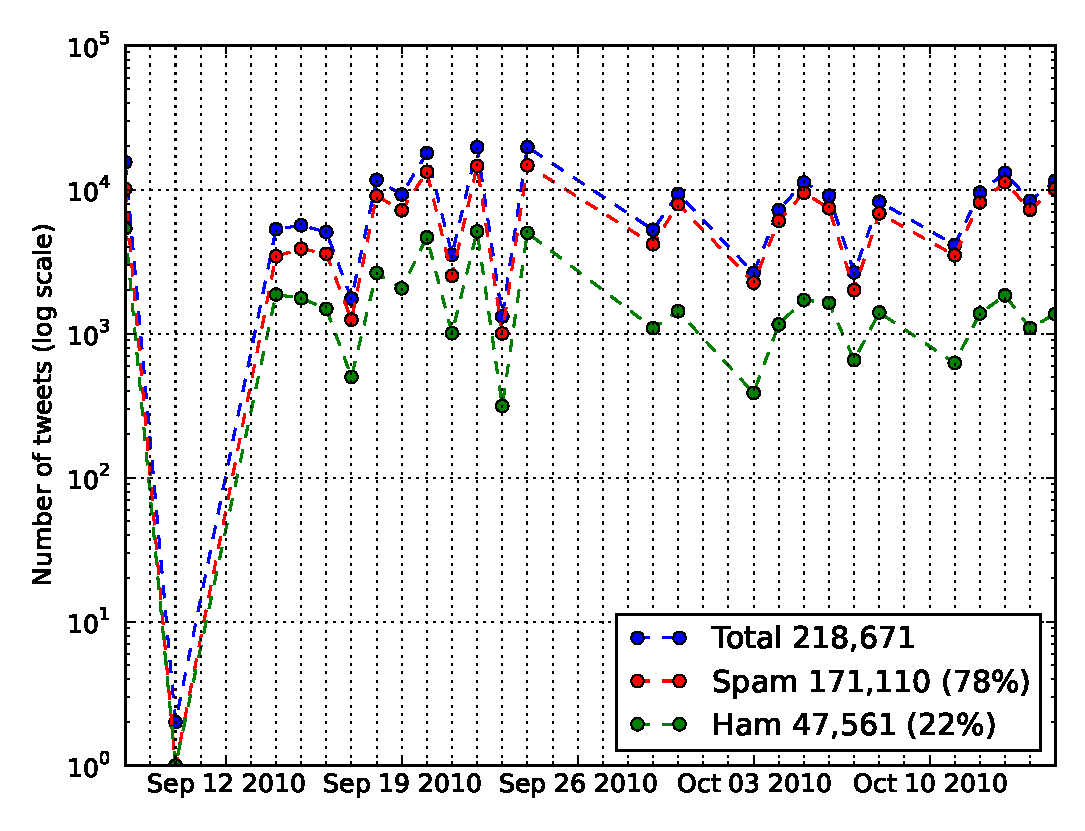
\includegraphics[width=8.8cm]{tweets_per_day.eps}
	\caption{The working dataset. Notice the non-contiguous days messages are present,
	the high proportion of spam tweets and the general non-uniformity of the number of
	messages per day. Since we do not use timing features, we do not expect this to
	be an issue.}
	\label{sample}
\end{figure}


We distilled a subset of the features of this data for our study. Focusing on content features, 
we examined records for the tweet messages and crawled HTML content. It is worth noticing that
there is a one to many mapping between a tweet and distinct HTML contents, for two reasons. First, 
a tweet might contain more than one URL, and second, one URL might lead to several distinct HTMLs
because of pop-ups. Figure \ref{sample} summarizes the most salient features of the sample. 78\% of the 0.22m
messages are labeled as spam, the compressed data holds in about 1Gb, the plain data occupies 25Gb
\footnote{We actually never need to decompress the \texttt{tar.gz} file as one can sequentially 
stream through the contained files.}.

\section{Language detection for tweets}
In order to limit our preliminary results to those that we could interpret, we further filtered 
this data to include only English language tweets. Our first attempt was to naively use the API data provided
by twitter, however we soon found out that the quality of the language labels was insufficient.
It turns out that language detection for short runs of characters is a difficult problem~\cite{Vojtek2007}~\cite{Gottron2010}
~\cite{Carter2011}. We decided to create our very own language detection algorithm and to build it
on the solid grounds of information theory. More precisely, we adopted the universal 
compression based approach~\cite{Li2008}.

We briefly describe our algorithm, which is both important and incidental to our method. 
The general idea is as follows. If $x$, $y$ and $z$ are three strings and $C$ is a lossless compressor, for example
an off-the-shelf compressor such as zip, tar, rar, lzma, \dots, then $x$ is more similar to $y$ than to $z$ if
$|C(yx)|-|C(y)| < |C(zx)|-|C(z)|$, where $yx$ is the concatenation of strings $x$ and $y$, and $|.|$ denotes the size 
of an object measured in bits. In other words, if $x$ is better compressed knowing data $y$ than knowing data $z$, $x$ is
closer to $z$. For example, if $x=$ \verb ababcababacab , $y=$ \verb ababababbaabab , $z=$ \verb cbacabcacacacb , then a
good compressor $C$ should pick up the repeating \verb ab  pattern in both $x$ and $y$ and provide a better compression
of $x$ given $y$ than given $z$. The notion of Kolmogorov complexity~\cite{Li2008} formalizes this intuition.

Our algorithm works by compressing the input against different language corpora and outputs the corpora which minimizes
the size in bits of the compressed output. More specifically, we use the prediction by partial matching~\cite{Cleary1984} approach, where 
the next character to occur is predicted by its immediate context of preceding $n$-characters. In effect, the algorithm 
works in two phases, the first phase being the training phase and occurs once and for all.
\begin{enumerate}
	\item In the learning phase, we train the predictors of the form $x_1\dots x_{n-1} \rightarrow x_n (\alpha_{x_1 \dots x_n})$
		(character $x_n$ occurs with probability $ \alpha_{x_1 \dots x_n}$ in context $x_1\dots x_{n-1}$) for all the languages
		corpora. In practice, we use plain UTF-8 ebooks from the Project Gutenberg~\cite{Gutenberg}.
	\item In the normal usage phase, we compute the number of bits needed for compressing the given instance using the predictors 
		of each language by simulating the compression and encoding operation. In practice, this operation is quite fast 
		with the proper pointer structure for matching partial contexts.
\end{enumerate}
The method has two downsides. First, it requires storing the predictors in memory all the time. This amounts to about 20Mb for the 13 
languages we trained our algorithm on. Pruning the predictors tree can help in that respect. Second, the algorithm is essentially a 
tournament between all the languages, with no clear notion of uncertainty about the output. We only know the difference in bits 
between the winner corpus and the one immediately below. This is why we so far only claim good performances on the task of 
detecting tweets in English.

\begin{figure}[!h]\centering
	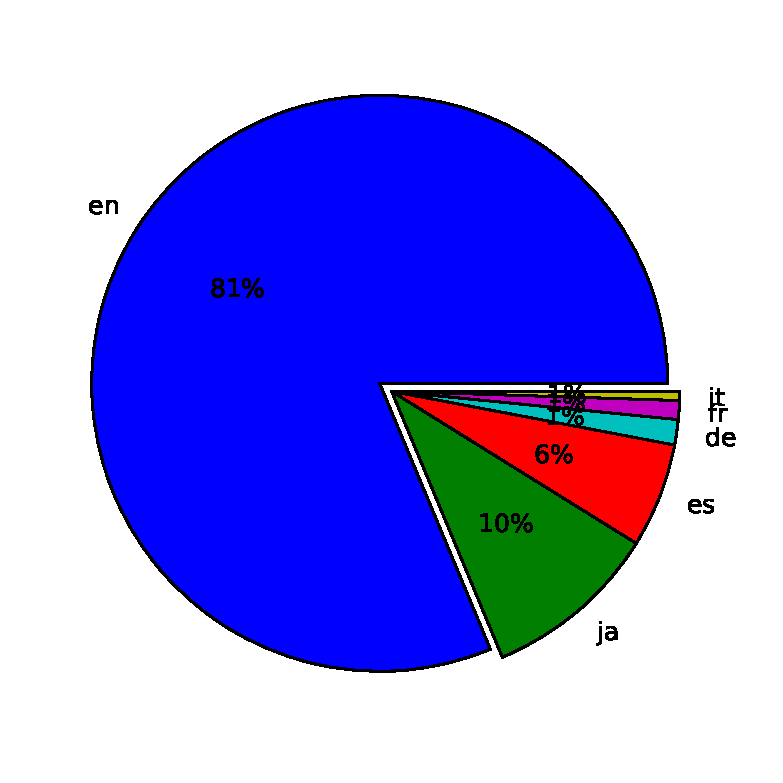
\includegraphics[width=8.5cm]{lang_twitter.eps}
	\caption{Languages distribution according to Twitter.}
	\label{tw_lang}
\end{figure}

\begin{figure}[!h]\centering
	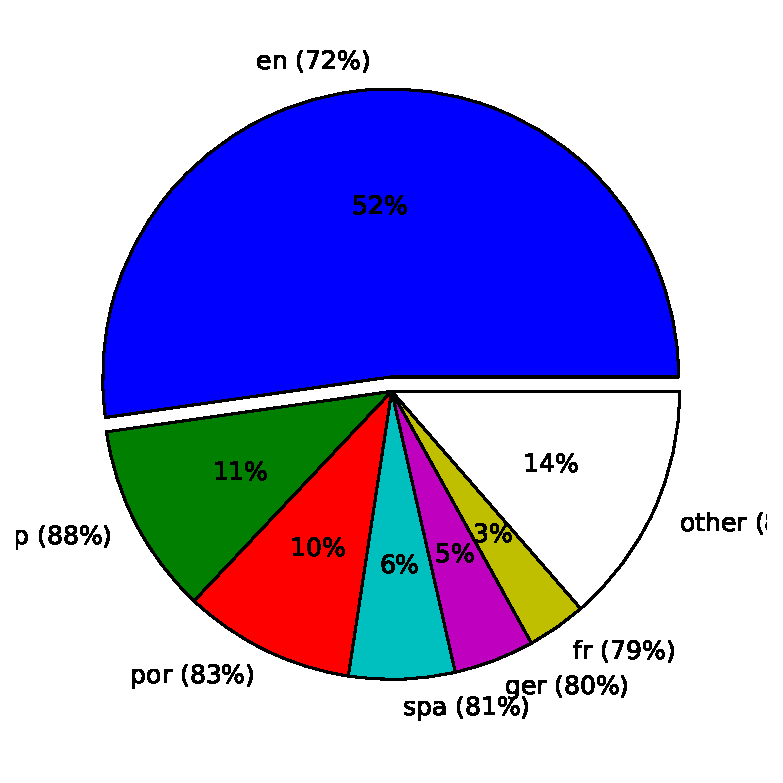
\includegraphics[width=8.5cm]{lang_infered.eps}
	\caption{Languages distribution according to the compression algorithm. The percentages following languages names 
		represent the proportion of spam in the given language.}
	\label{inf_lang}
\end{figure}

A hand labeling of about a 100 tweets shows that our algorithm achieves more than 99\% precision and recall for English tweets. Figures
\ref{tw_lang} and \ref{inf_lang} respectively show Twitters' labeling and our labeling (after cleaning-up the tweets contents 
as described in what follows), where rarely occurring languages have been collapsed
together. This category contains languages like Dutch, Norwegian, Russian, Chinese, some Tagalog, and some 
obvious miscategorizations such as Latin.

\section{Topic modeling on twitter}

We began our study with the hope to improve classification accuracy of Monarch by deriving higher-level content features from those that Monarch collects.
The two main advantages of topic modeling with LDA over other methods of processing text for classification based on word frequency are:
\begin{enumerate}
\item the identification of synonyms and disambiguation of homographs based on document context
\item the explanatory power of the reduced feature space, which often captures intuitive categories of behavior or communication. 
\end{enumerate}
We expected that LDA will learn categories of activity that we pick out with ease perceptually, such as Viagra ads, consumer electronics affiliates, and domain squatting.
We aimed to apply LDA to the content features of the messages and crawled URLs in the available data to derive new features for spam filtering.

At a high level, topic modeling with LDA involves:
\begin{enumerate}
\item Preparing corpus data to be consumed by LDA
\item Training the topic model on the corpus.  Each `topic' is a distribution over words that captures the statistical co-occurrence of tokens.
\item Evaluating documents against the topic model to get an estimated topic mixture per document.  This mixture will be the distribution over topics that is most likely to have generated the document, given the model.
\end{enumerate}

In the next section we will describe how we used documents' topic mixtures to investigate link deception.
In this section, we will describe the topic modeling process itself.


\subsection{Preparing data for topic modeling}

For the purposes of our study, 'documents' are either tweet messages or HTML pages.
However, the peculiarities of LDA necessitate a significant amount of preprocessing on this raw content in order to be effective.

\subsubsection{Bags of words}

LDA uses a ``bag of words'' model for documents.
This means that word order is ignored in LDA.
Rather, words are tokenized from records in the corpus and stored sparsely as a feature matrix associating an occurrence count with each token.

\subsubsection{Stop word removal}

LDA fits the parameters of its topic model to reflect the composition of documents in the provided corpus.
For very frequently occurring words, however, the words presence does not provide any information about the documents contents or meaning.
Typical examples of these ``stop words'' in English include ``a'', ``and'', and ``it''.
It is common practice to remove these stop words when preparing documents for consumption by LDA.
Several open source packages for performing LDA will do this automatically.

For our study, we needed to go beyond the typical list of English stop words to account for uninformative tokens in our particular domains.
For twitter messages, we removed idiomatic tokens such as ``RT'' (\emph{retweet}) and ``FF'' (\emph{follow friday}).
In the HTML pages, we removed common HTML tags.


Data cleaning 

stopword removal



Vern says: Your writeup should make some things clear that here weren't so much, such as just what constitutes a "document" (a single tweet? that appeared to be the meaning), how LDA works (don't assume I know - because I don't!), what you mean by "parsity" (sparsity?), and what the reader is supposed to make of the      LDA output in the appendix.

LDA implementations operate on documents


Our  goal for the first segment of our research was to train a classifier  based on learned topics from the data and troubleshoot the process along  the way.

Focusing on the tweet messages themselves, we cleaned this data by generating a list of stopwords based on commonly used English stopwords as well as informally based on observed term frequency in order to account for the peculiarities of Twitter lexical feature frequency.

Running the standard LDA algorithm on these short messages produced two results:
	* A list of topics, labeled with 'topic keys'  the most prominent words used in the topics
	* An inferred distribution of topics per document
    
The results from the topic keys were promising, with several of the topics corresponding to domain knowledge of what constitutes spam.  For example. one topic was characterized by these keywords:

news world iphone win tv apple google watch ipad ap hey  app price search sports click buy giveaway case ipod late shows gb touch  tech test year deal series 

Using the topic distribution for each document as a feature vector, we trained a naive Bayes classifier and tested its spam detection accuracy against the labeled data, using n-fold cross validation.

The performance of this classifier was underwhelming (.57 accuracy against a spam base rate of .73).  However, this is unsurprising given the parsity of data we were using for this particular iteration.
\subsection{Clean-up process}


\begin{figure}
	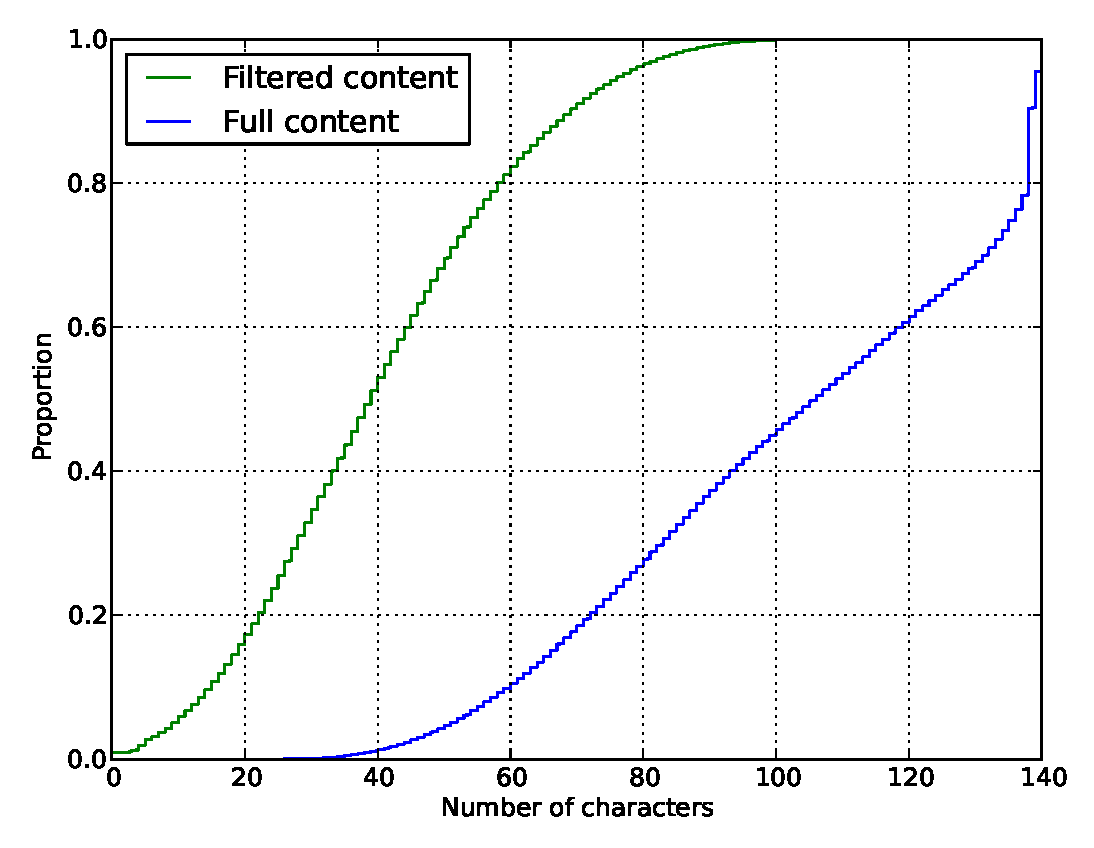
\includegraphics[width=8.8cm]{cdf_en_content_length.eps}
	\caption{Effect of cleaning up code on content length. The cumulative probability distributions of content length
	for both cleaned up and raw tweets are plotted.}
	\label{len_cdf}
\end{figure}

\section{Detecting deceptive tweets}

\begin{figure*}[ht]\centering
	\begin{subfigure}[c]{8.8cm}
	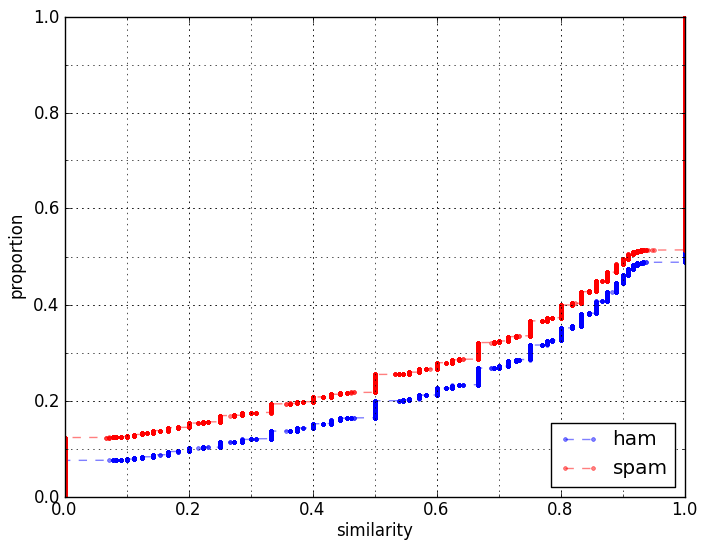
\includegraphics[width=8.8cm]{jacc_max.png}
	\caption{Jaccard similarity.}
	\end{subfigure}
	\begin{subfigure}[c]{8.8cm}
	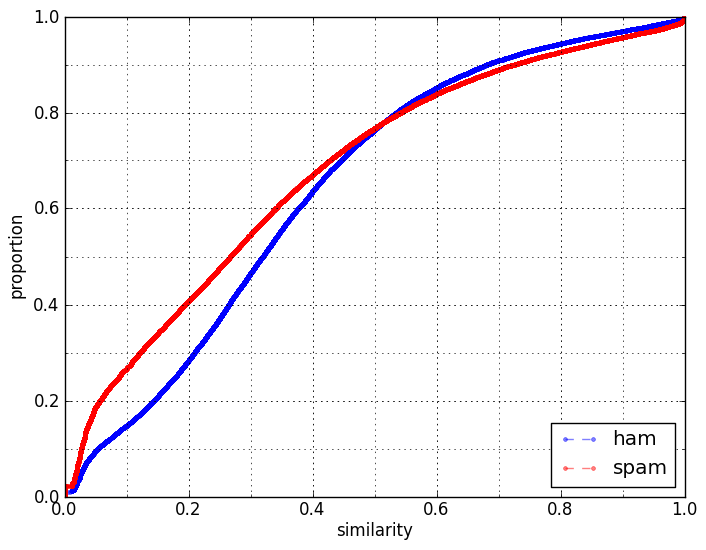
\includegraphics[width=8.8cm]{cosine_lda10_max.png}
	\caption{LDA-10 cosine similarity.}
	\end{subfigure}
	\caption{Cumulative probability distributions for the
		naive Jaccard similarity measure and the 10 topics LDA
		with cosine distance. Notice the discretized values of the
		Jaccard measure and the continuous values of the LDA
	based method.}
\end{figure*}

In this part, we focus on determining a good similarity measure between tweet content and linked content. To this end, we make use of the spam labeling, with the assumption we will further verify that ham tweets display more similarity than spam tweets. Our approach is as follows:
\begin{enumerate}
	\item We define a set of candidate similarity measures.
	\item We evaluate each of the candidates using the spam labeling in the dataset.
	\item We a posteriori validate or invalidate the results by manually looking at low-similarity and high-similarity tweets.
\end{enumerate}

\subsection{Candidate similarity measures}
We thereby define 3 similarity measures. A similarity measure is any function which takes for input two strings and return a value between 0 and 1.

\subsubsection{Naive Jaccard measure}
The naive Jaccard measure between a tweet $T$ and its linked HTML content $H$ is defined by:
\[
	\simil_{J}(T, H) = \frac{|\bow(T) \cap \bow(H)|}{|\bow(T)|}
\]
where $\bow$ is the bag-of-wording function which takes a string and returns a set of normalized tokens with stop words removed. This measure is expected to perform relatively poorly because of the sparse, high dimensional nature of the bag of words. We expect a lot of blunt 0 and 1 values for this metric.

\subsubsection{TF-IDF normalized cosine measure}
The TF-IDF distance 

\begin{table}[!h]\centering
	\begin{tabular}{|c|p{1.5cm}|p{1cm}|p{1cm}|p{1cm}|}
	\hline
	Projection & Similarity measure & min AUC & max AUC & avg AUC \\
	\hline
	None & Jaccard & 0.393 & 0.395 & 0.395 \\
	TF-IDF & Cosine & 0.102 & 0.102 & 0.102 \\
	LDA-5 & Cosine & 0.531 & 0.533 & 0.532 \\
	LDA-10 & Cosine & 0.552 & 0.556 & 0.554 \\
	LDA-20 & Cosine & 0.549 & 0.552 & 0.551 \\
	LDA-40 & Cosine & 0.446 & 0.450 & 0.450 \\
	\hline
	\end{tabular}
	\label{perf}
	\caption{AUC measures for different similarity measures when used 
		as a spam detector by thresholding on the similarity. LDA with
		10 topics is the best candidate, TF-IDF performs particularly
	badly on the task.}
\end{table}

\begin{figure}[ht]\centering
	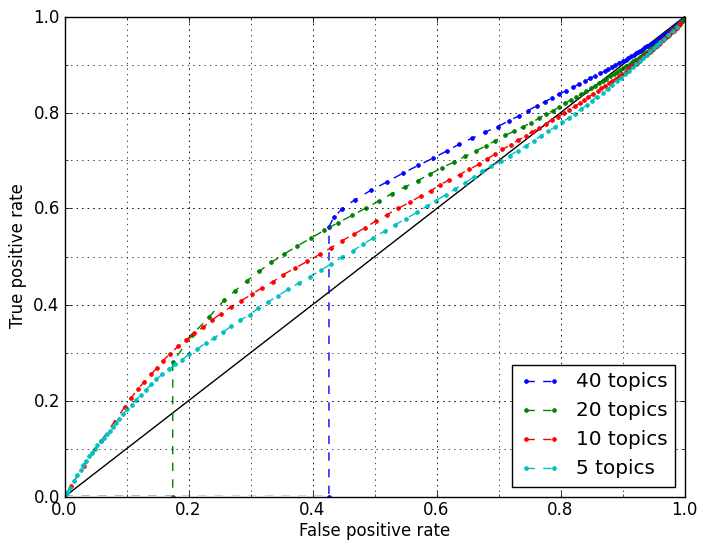
\includegraphics[width=8.8cm]{roc_lda_sim.png}
	\caption{ROC curves of the hypothetical spam filters based on thresholding k-topics LDA cosine
	similarity. Notice the sudden drops at higher dimensions as the data sparsity comes into play.}
\end{figure}
\subsection{A closer look at the data}

\section{Discussion}


\section{Conclusion}
Future work.

\bibliography{collection.bib}
\bibliographystyle{ieeetr}
\end{document}
